%!TEX root = first try.tex

\chapter{Case study}

A case study to assess the feasibility of the methods/criteria developed in previous paragraphs by using both FEM software and methods/criteria. 


\chapter{Conclusion}

%Compare the result from different calculation method. Give conclusion based on the comparison result.

\begin{appendices}
\chapter{Frequency and wavelength data used in D181 DT 329}

\begin{table}[h]
    \centering
    \begin{tabular}{c|c|c|c}
    \hline
    \multirow{2}{*}{Freight train: Principle axle repeat patterns} & dist & \multicolumn{2}{c}{Speed} \\
    & m & 60 km/h & 100 km/h \\
    \hline
    wagon n axle 2 - wagon n+1 axle 1 & 4.00 & 4.17 & 6.94 \\
    wagon wheelbase & 9.00 & 1.85 & 3.09 \\
    wagon n axle m - wagon n+1 axle m & 13.0 & 1.28 & 2.14 \\
    wagon n axle m - wagon n+2 axle m & 26.0 & 0.64 & 1.07 \\
    \hline
    \multirow{2}{*}{Passenger train: Principle axle repeat patterns} & dist & \multicolumn{2}{c}{Speed} \\
    & m & 160 km/h & 200 km/h \\
    \hline
    coach n axle 1 - 2, and coach n axle 3 - 4 & 2.56 & 17.36 & 21.70 \\
    coach n axle m - coach n+1 axle m & 26.4 & 1.68 & 2.10 \\
    coach n axle m - coach n+2 axle m & 52.8 & 0.84 & 1.05 \\
    \hline
    \multirow{2}{*}{ETR 500 train: Principle axle repeat patterns} & dist & \multicolumn{2}{c}{Speed} \\
    & m & 300 km/h & 350 km/h \\
    \hline
    coach n axle 1 - 2 and coach n axle 3 - 4 & 3.0 & 27.78 & 32.41 \\
    coach n axle m - coach n+1 axle m & 26.1 & 3.19 & 3.72 \\
    coach n axle m - coach n+2 axle m & 52.2 & 1.60 & 1.86 \\
    coach n axle m - coach n+3 axle m & 69.3 & 1.20 & 1.40 \\
    \hline
    \end{tabular}
    \caption{Axle repeat patterns and typical frequencies. Extracted from \cite[Appendix C]{d181dt329}}
    \label{tab:329axlerepeat}
\end{table}

\begin{table}[h]
    \centering
    \begin{tabular}{c|c|c|c}
    \hline
    Kinematic wavelength, m & Freight train & Passenger train & ETR500 train \\
    \hline
    Locomotive & 39 - 45 & 32 - 38 & 39 - 45 \\
    Coach/wagon & 24 - 39 & 34 - 38 & 36 - 40 \\
    \hline
    \end{tabular}
    \caption{Kinematic wavelength ranges per vehicle, with BR P1 profiles. Extracted from \cite[Appendix C]{d181dt329}}
    \label{tab:329kinematicwavelength}
\end{table}

\chapter{Speeds which do not require dynamic compatibility checks} \label{app:speedsafe}

\begin{figure}[h]
    \centering
    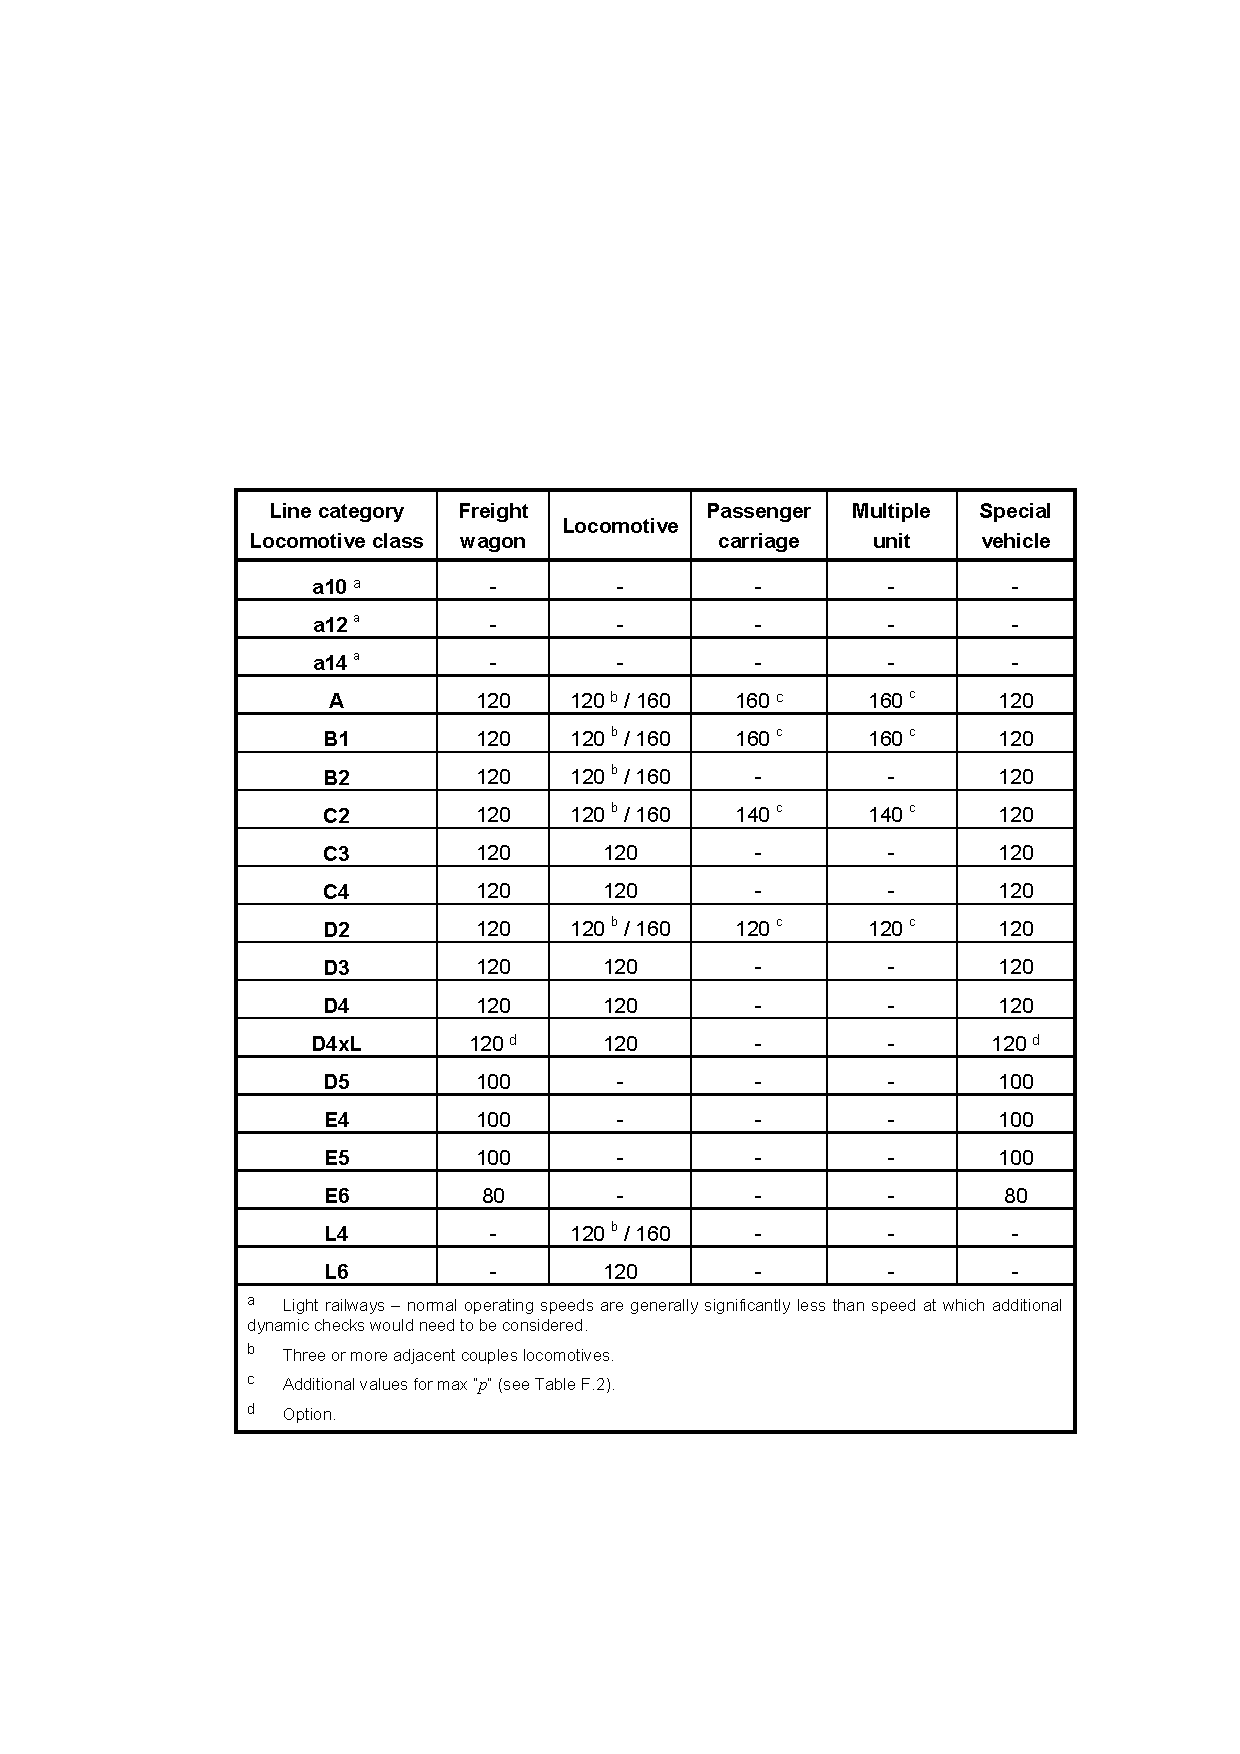
\includegraphics[width=0.7\textwidth]{speedsafe.pdf}
    \caption{Speed limit (in km/h) in relationship Line Category/Locomotive Class and vehicle type. Extract from \cite[Appendix F]{EC15528}}
\end{figure}

\chapter{MU-Groups and MU-Classes}\label{app:mu}

\section{Definition}
Multiple units can be grouped according to type of traffic service(high speed - long distance, intercity - regional and commuter/suburban) or to the kind of running gear (conventional bogies, articulated bogies and single axles).


In some cases due to potential excessive dynamic load effects in bridge line category checks are not sufficient to demonstrate compatibility. To minimise the need for undertaking a dynamic check of individual trains, several typical and wide spread MU-designs have been grouped in MU-classes. For these groups of vehicles, load models covering the specified design parameter ranges have been developed to allow the efficient dynamic analysis of bridges. For practical reasons, the number of MU classes was limited and for trains outside the range of parameters covered, the process of checking an individual train existing at the time of publication of this standard as state of the art shall be used.

Each MU-class is defined by:

\begin{enumerate}[-]
\item ranges of train parameters covered and;
\item a corresponding load model for carrying out dynamic checks on bridges.
\end{enumerate}

Each MU-Group comprises of serveral MU-Classes. Table

\begin{table}[h]
    \centering
    \begin{tabular}{c|c}
        \hline
        MU-Group & MU-Class\\
        \hline
        \multirow{2}{*}{conventional bogie(CB)} & $CB_1$ \\
        & $CB_2$ \\
        \hline
        \multirow{4}{*}{articulated bogie(AB)} & $AB_1$ \\
        & $AB_2$ \\
        & $AB_3$ \\
        & $AB_4$ \\
        \hline
        \multirow{2}{*}{single axle(SA)} & $SA_1$ \\
        & $SA_2$ \\
        \hline
    \end{tabular}
    \caption{Relationship MU-groups - MU-classes}
    \label{tab:MU}
\end{table} 

\begin{figure}[h]
\centering
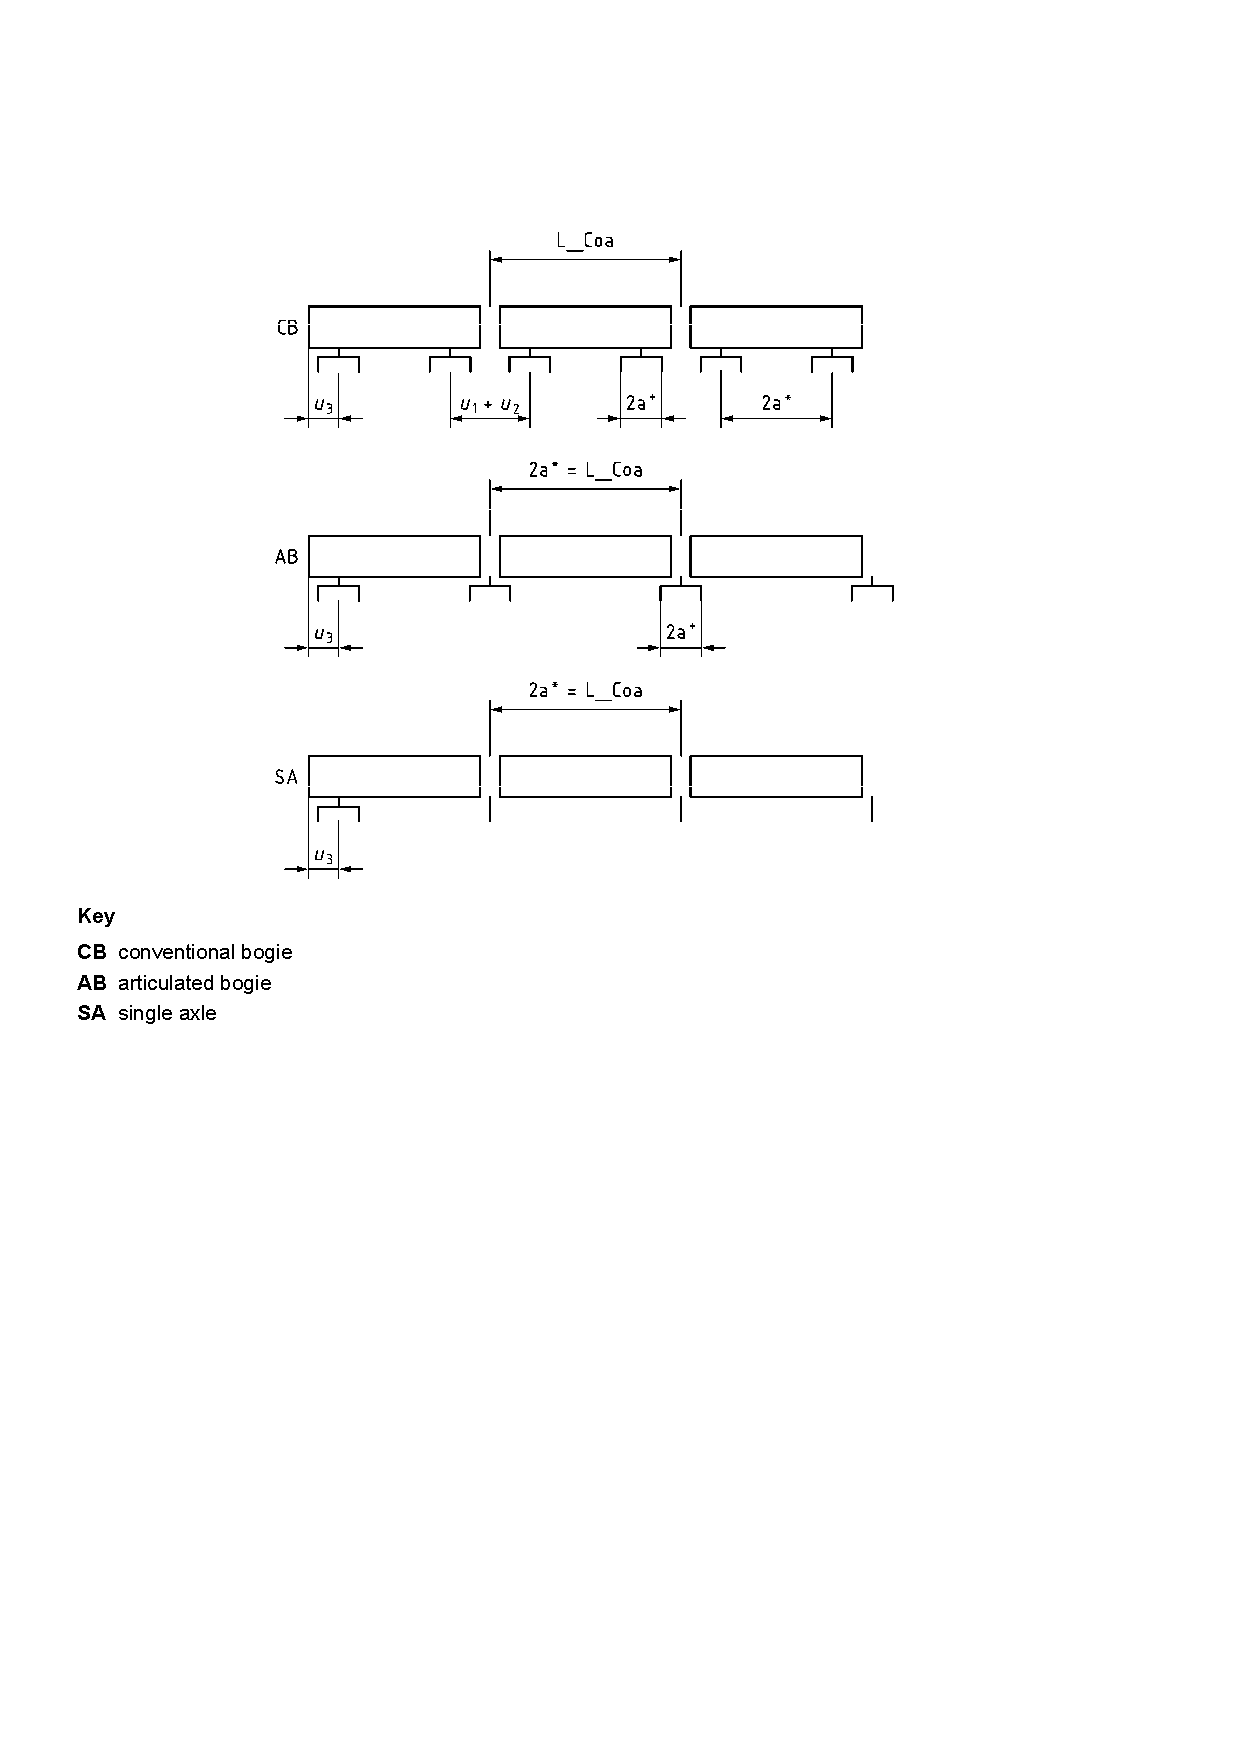
\includegraphics[width=0.8\textwidth]{trainparameters.pdf}
\caption{Train parameters related to MU-Groups. Extracted from \cite[Annex C]{EC15528}}
\label{fig:trainparameters}
\end{figure}

\begin{table}[h]
    \centering
    \begin{tabular}{c|c|c}
    \hline
    Name & Parameter & Unit \\
    $2a^*$ & Bogie spacing between pivot centres within a vehicle & m \\
    $2a^+$ & Axle spacing in bogie & m \\
    $u1+u2$ & Bogie spacing between pivot centres of adjacent vehicles & m \\
    $u3$ & Overhang of end coaches & m \\
    L\_Coa & Coach length & m \\
    No\_Coa & Number of coaches within an unit & - \\
    No\_Units & Number of units within a train & - \\
    \hline
    \end{tabular}
    \caption{Explanation of train parameters. Extracted from \cite[Annex C]{EC15528}}
    \label{tab:explanationtrainparameters}
\end{table}

\subsection{Train parameters of MU-Class CB\_1}

\begin{table}[h]
    \centering
    \begin{tabular}{c|c}
    \hline
    max No\_Units & 2 \\
    max No\_Coa & 8 \\
    L\_Coa & $23.8m \leq L\_Coa \leq 25.3m $ \\
    $2a^*$ & $16.8m \leq 2a^* \leq 18.0m $ \\
    $2a^+$ & $2m \leq 2a^+ \leq 3m $ \\
    $(u1+u2)$ & $7.0m \leq (u1+u2) \leq 7.6m $ \\
    $u3$ & $4m \leq u3 \leq 6m $ \\
    \hline
    \end{tabular}
    \caption{Train parameters for conformity with MU-Class CB\_1}
    \label{tab:CB1}
\end{table}

\subsection{Train parameters of MU-Class CB\_2}

\begin{table}[h]
    \centering
    \begin{tabular}{c|c}
    \hline
    max No\_Units & 2 \\
    max No\_Coa & 7 \\
    L\_Coa & $ 25.3 m \leq L\_Coa \leq 27.5 m $ \\
    $2a^*$ & $ 18.0 m \leq 2a^* \leq 19.5 m $ \\
    $2a^+$ & $ 2 m \leq 2a^+ \leq 3m $ \\
    $(u1+u2)$ & $7.2m \leq (u1+u2) \leq 8.0 m $ \\
    $u3$ & $4m \leq u3 \leq 6m $ \\
    \hline
    \end{tabular}
    \caption{Train parameters for conformity with MU-Class CB\_2}
    \label{tab:CB2}
\end{table}


\subsection{Train parameters of MU-Class AB\_1}

\begin{table}[h]
    \centering
    \begin{tabular}{c|c}
    \hline
    max No\_Units & 4 \\
    max No\_Coa & 5 \\
    $2a^*$ & $ 14.9 m \leq 2a^* \leq 16.0 m $ \\
    $2a^+$ & $ 2 m \leq 2a^+ \leq 3m $ \\
    $u3$ & $3m \leq u3 \leq 5.5m $ \\
    \hline
    \end{tabular}
    \caption{Train parameters for conformity with MU-Class AB\_1}
    \label{tab:AB1}
\end{table}

\subsection{Train parameters of MU-Class AB\_2}

\begin{table}[h]
    \centering
    \begin{tabular}{c|c}
    \hline
    max No\_Units & 4 \\
    max No\_Coa & 5 \\
    $2a^*$ & $ 18.8 m \leq 2a^* \leq 19.5 m $ \\
    $2a^+$ & $ 2 m \leq 2a^+ \leq 3m $ \\
    $u3$ & $3m \leq u3 \leq 5.5m $ \\
    \hline
    \end{tabular}
    \caption{Train parameters for conformity with MU-Class AB\_2}
    \label{tab:AB2}
\end{table}

\subsection{Train parameters of MU-Class AB\_3}

\begin{table}[h]
    \centering
    \begin{tabular}{c|c}
    \hline
    max No\_Units & 2 \\
    max No\_Coa & 11 \\
    $2a^*$ & $ 17.0 m \leq 2a^* \leq 17.5 m $ \\
    $2a^+$ & $ 2 m \leq 2a^+ \leq 3m $ \\
    $u3$ & $4.5m \leq u3 \leq 5.7m $ \\
    \hline
    \end{tabular}
    \caption{Train parameters for conformity with MU-Class AB\_3}
    \label{tab:AB3}
\end{table}

\subsection{Train parameters of MU-Class AB\_4}

\begin{table}[h]
    \centering
    \begin{tabular}{c|c}
    \hline
    max No\_Units & 2 \\
    max No\_Coa & 10 \\
    $2a^*$ & $ 18.7 m \leq 2a^* \leq 19.2 m $ \\
    $2a^+$ & $ 2 m \leq 2a^+ \leq 3m $ \\
    $u3$ & $4.3m \leq u3 \leq 5.3m $ \\
    \hline
    \end{tabular}
    \caption{Train parameters for conformity with MU-Class AB\_4}
    \label{tab:AB4}
\end{table}

\subsection{Train parameters of MU-Class SA\_1}

\begin{table}[h]
    \centering
    \begin{tabular}{c|c}
    \hline
    max No\_Units & 3 \\
    max No\_Coa & 10 \\
    $2a^*$ & $ 9.2 m \leq 2a^* \leq 9.8 m $ \\
    $u3$ & $4.25m \leq u3 \leq 6.25m $ \\
    \hline
    \end{tabular}
    \caption{Train parameters for conformity with MU-Class SA\_1}
    \label{tab:SA1}
\end{table}

\subsection{Train parameters of MU-Class SA\_2}

\begin{table}[h]
    \centering
    \begin{tabular}{c|c}
    \hline
    max No\_Units & 2 \\
    max No\_Coa & 14 \\
    $2a^*$ & $ 12.8 m \leq 2a^* \leq 13.5 m $ \\
    $u3$ & $4.25m \leq u3 \leq 6.25m $ \\
    \hline
    \end{tabular}
    \caption{Train parameters for conformity with MU-Class SA\_1}
    \label{tab:SA1}
\end{table}

\end{appendices}